\documentclass[11pt, a4paper]{article}

% ─── PAQUETES ─────────────────────────────────────────────────────────────────
\usepackage[utf8]{inputenc}
\usepackage[T1]{fontenc}
\usepackage[spanish,es-tabla,es-noshorthands]{babel}
\usepackage{geometry}
\geometry{top=2.4cm, bottom=2.4cm, left=2.6cm, right=2.6cm, headheight=15pt}

\usepackage{amsmath, amssymb}
\usepackage{graphicx}
\usepackage{booktabs}
\usepackage{array}
\usepackage{multirow}
\usepackage{xcolor}
\usepackage{hyperref}
\usepackage{float}
\usepackage{caption}
\usepackage{enumitem}
\usepackage{fancyhdr}
\usepackage{titlesec}
\usepackage{parskip}
\usepackage{tikz}
\usetikzlibrary{arrows.meta, positioning}

\captionsetup{font=small, labelfont=bf}
\setlist{nosep, leftmargin=1.2em}

% ─── COLORES ──────────────────────────────────────────────────────────────────
\definecolor{azuloscuro}{RGB}{13, 71, 161}
\definecolor{azulclaro}{RGB}{227, 242, 253}

\hypersetup{colorlinks=true, linkcolor=azuloscuro, citecolor=azuloscuro, urlcolor=azuloscuro}

% ─── ENCABEZADO ───────────────────────────────────────────────────────────────
\pagestyle{fancy}
\fancyhf{}
\fancyhead[L]{\small\textcolor{azuloscuro}{\textbf{Naïve Bayes y noticias financieras}}}
\fancyhead[R]{\small\textcolor{azuloscuro}{Wall Street Pulse}}
\fancyfoot[C]{\thepage}
\renewcommand{\headrulewidth}{0.5pt}

% ─── SECCIONES ────────────────────────────────────────────────────────────────
\titleformat{\section}{\large\bfseries\color{azuloscuro}}{\thesection.}{0.5em}{}[\color{azuloscuro}\titlerule]
\titleformat{\subsection}{\normalsize\bfseries\color{azuloscuro!80}}{\thesubsection.}{0.5em}{}
\titlespacing*{\section}{0pt}{1.2ex}{0.8ex}
\titlespacing*{\subsection}{0pt}{1ex}{0.5ex}

\begin{document}

% ╔══════════════════════════════════════════════════════════════════════════════╗
\begin{center}
    \vspace*{0.3cm}
    {\LARGE\bfseries\color{azuloscuro}
        Clasificación del Impacto de Noticias Financieras\\[0.2em]
        con Naïve Bayes Multinomial\par}
    \vspace{0.5em}
    \rule{0.85\textwidth}{1pt}\\[0.4em]
    {\large\itshape Del titular al nivel de impacto: un flujo de procesamiento de texto en R
    y el diagnóstico de un conjunto de datos sin señal\par}
    \vspace{0.8em}
    {\normalsize
    Juan Pablo Venegas Padilla \quad\textbullet\quad Arie Zalo González\\[0.25em]
    Santiago de la Calleja Jiménez \quad\textbullet\quad Juan Pablo Espinosa Maciel\par}
    \vspace{0.3em}
    {\small Ingeniería en Ciencia de Datos y Matemáticas, Tecnológico de Monterrey\\[0.15em]
    \today\par}
    \vspace{0.8em}
    \colorbox{azulclaro}{%
        \parbox{0.92\textwidth}{\small
            \vspace{0.2cm}
            \textbf{Resumen.} Este trabajo construye un clasificador \textbf{naïve Bayes
            multinomial} que estima el nivel de impacto de una noticia financiera a partir de su
            titular, sobre un conjunto de 3{,}024 noticias con evento de mercado, sector,
            sentimiento e indicadores del índice asociado. La metodología encadena un análisis
            exploratorio y una limpieza en Python con un flujo de procesamiento de texto en R:
            tokenización de los titulares, eliminación de palabras vacías, construcción de una
            matriz dispersa documento--término, recodificación de la variable objetivo a dos
            clases —impacto alto contra impacto medio o bajo— y ajuste del clasificador con
            suavizado de Laplace sobre una partición de 80/20. El resultado es un modelo que
            \textbf{no supera a la regla trivial} de predecir siempre la clase mayoritaria: su
            exactitud queda por debajo de esa línea base, dos de cada tres alertas de impacto alto
            son falsas y más de la mitad de las noticias realmente relevantes pasan desapercibidas.
            La explicación no está en el clasificador sino en los datos, y el análisis exploratorio
            la anticipa: el conjunto contiene apenas 50 titulares distintos repetidos decenas de
            veces, un mismo titular aparece etiquetado con los tres niveles de impacto, y ni el
            sentimiento ni los indicadores numéricos discriminan entre niveles. Asignar a cada
            titular su etiqueta más frecuente acierta solo un 41\,\%, de modo que el techo de
            cualquier modelo que use únicamente el texto está fijado de antemano. El aporte del
            trabajo es doble: un flujo reproducible de clasificación de texto financiero, y el
            diagnóstico documentado de por qué un conjunto puede impedir el aprendizaje por
            construcción.
            \vspace{0.2cm}}}
    \vspace{0.4em}

    {\small\textbf{Palabras clave---} Naïve Bayes multinomial, clasificación de texto, noticias
    financieras, bolsa de valores, matriz documento--término, suavizado de Laplace, ruido de
    etiquetas.\par}
    \vspace{0.6em}
\end{center}

% ─── 1. INTRODUCCIÓN ──────────────────────────────────────────────────────────
\section{Introducción}

Que las noticias mueven los mercados es una de las pocas afirmaciones que casi nadie discute en
finanzas. Lo que sí se discute es cuánto y en qué dirección, y la evidencia empírica al respecto
proviene en buena medida del análisis del texto: Tetlock \cite{tetlock2007} mostró que el tono
pesimista de una columna diaria del \textit{Wall Street Journal} anticipa presión a la baja en los
precios y un repunte posterior del volumen, y Loughran y McDonald \cite{loughran2011} documentaron
que los diccionarios de sentimiento diseñados para textos generales clasifican mal el lenguaje
financiero, al punto de que casi tres cuartas partes de las palabras que un diccionario estándar
considera negativas no lo son en un informe corporativo.

Si el texto de una noticia contiene información sobre el mercado, la pregunta operativa para
quien invierte es más simple que la académica: dado el titular que acaba de publicarse, ¿esta
noticia va a mover el índice de forma apreciable o no? Formulada así, es un problema de
clasificación de texto, y el clasificador natural para empezar es \textbf{naïve Bayes}. Este
trabajo lo construye y lo evalúa sobre un conjunto de noticias financieras etiquetadas con su
nivel de impacto.

\subsection{Antecedentes y estado del arte}

Naïve Bayes es un clasificador probabilístico que estima la probabilidad de cada clase dado el
documento suponiendo que las palabras son condicionalmente independientes entre sí una vez fijada
la clase. En finanzas tiene un antecedente directo: Antweiler y Frank \cite{antweiler2004}
clasificaron más de un millón y medio de mensajes de foros bursátiles con naïve Bayes y
encontraron que, si bien el efecto sobre los rendimientos es económicamente pequeño, el desacuerdo
entre mensajes predice volatilidad y volumen. Es decir, el enfoque de bolsa de palabras aplicado a
texto financiero no es una curiosidad metodológica sino una herramienta con historial.

En clasificación de texto en general, el modelo multinomial —que representa cada documento por el
número de veces que aparece cada término del vocabulario— es la formulación de referencia
\cite{manning2008}. McCallum y Nigam \cite{mccallum1998} compararon sistemáticamente esa
formulación contra la alternativa de Bernoulli, que solo registra presencia o ausencia, y
concluyeron que la multinomial rinde mejor en vocabularios grandes, que es la situación habitual.
Su atractivo persistente es que el supuesto de independencia, que casi nunca se cumple en lenguaje
natural, no impide un buen desempeño: Domingos y Pazzani \cite{domingos1997} explicaron por qué un
clasificador puede acertar la clase aunque sus estimaciones de probabilidad estén sesgadas, ya que
para decidir basta con ordenar bien las clases, no con calibrar sus probabilidades.

Hay, sin embargo, un límite que ningún clasificador cruza. Cuando las etiquetas de entrenamiento
contienen ruido —cuando ejemplos idénticos aparecen con etiquetas distintas— el desempeño
alcanzable está acotado con independencia del algoritmo, y el ruido puede además degradar el
aprendizaje más allá de esa cota \cite{frenay2014}. Este trabajo termina siendo, en buena medida,
un caso de estudio de esa situación.

\subsection{Problema y preguntas de investigación}

El objeto de estudio es un conjunto de 3{,}024 noticias financieras en el que cada registro trae el
titular, el evento de mercado que lo origina, el índice y el sector afectados, el sentimiento
asignado, el cambio porcentual del índice, el volumen operado y una etiqueta de nivel de impacto
con tres valores. Las preguntas son tres:

\begin{enumerate}
    \item[\textbf{P1}] ¿Puede un clasificador naïve Bayes multinomial distinguir, a partir del
        titular, las noticias de impacto alto del resto?
    \item[\textbf{P2}] ¿Qué desempeño alcanza frente a la línea base trivial de predecir siempre la
        clase mayoritaria, y qué significan sus errores para quien tomaría decisiones con él?
    \item[\textbf{P3}] Si el desempeño es bajo, ¿la causa está en el clasificador o en los datos?
\end{enumerate}

\subsection{Objetivos}

\textbf{General:} implementar y evaluar un flujo completo de clasificación de texto —desde los
datos crudos hasta las métricas— que estime el nivel de impacto de una noticia financiera a partir
de su titular. \textbf{Específicos:} (i)~caracterizar el conjunto y decidir de forma explícita el
tratamiento de los valores faltantes; (ii)~construir la representación de texto que el modelo
multinomial requiere; (iii)~ajustar el clasificador con suavizado y evaluarlo sobre una partición
independiente; (iv)~interpretar los errores en términos financieros; y (v)~determinar si el
desempeño observado es atribuible al modelo o a la estructura de los datos.

\subsection{Aportaciones}

\begin{enumerate}
    \item Un \textbf{flujo reproducible} de clasificación de texto financiero que va del CSV crudo
        a las métricas, con la etapa de exploración y limpieza en Python y la de texto y modelado
        en R, y con cada decisión de tratamiento de faltantes escrita de forma explícita.
    \item Un \textbf{diagnóstico del conjunto de datos} que precede al modelo y anticipa su
        resultado: la escasa variedad de titulares, la inconsistencia de las etiquetas y la
        ausencia de relación entre el nivel de impacto y el resto de las variables.
    \item Una \textbf{lectura financiera de los errores}, que traduce la precisión y la
        sensibilidad del clasificador al costo concreto de actuar sobre sus alertas.
\end{enumerate}

% ─── 2. METODOLOGÍA ───────────────────────────────────────────────────────────
\section{Metodología}

\subsection{Arquitectura del flujo de trabajo}

El proyecto se divide en dos etapas con lenguajes distintos. La \textbf{exploración y limpieza}
corre en Python con \texttt{pandas} \cite{mckinney2010} sobre un cuaderno que produce un único
archivo intermedio con las columnas útiles y sin valores faltantes. El \textbf{procesamiento de
texto y el modelado} corren en R \cite{rcore2024} sobre dos documentos Quarto: el primero usa
\texttt{tidyverse} \cite{wickham2019} y \texttt{tidytext} \cite{silge2016} para tokenizar los
titulares y construir la matriz documento--término, y el segundo ajusta el clasificador con el
paquete \texttt{naivebayes} \cite{majka2019}. La Fig.~\ref{fig:metodologia} resume las cinco fases.
Todo el código está disponible en
\url{https://github.com/JuanPVenegas13/Wall-Street-Pulse}.

\begin{figure}[H]
\centering
\begin{tikzpicture}[
    block/.style={rectangle, draw=azuloscuro, thick, fill=white, text width=11cm,
                  minimum height=0.95cm, align=left, rounded corners=2pt, font=\small},
    arrow/.style={-{Stealth[scale=1.1]}, thick, azuloscuro}
]
\node (s1) [block] {\textbf{1. Análisis exploratorio}\\
    Estructura, variedad del texto, consistencia de las etiquetas y faltantes.};
\node (s2) [block, below=0.42cm of s1] {\textbf{2. Limpieza y selección de columnas}\\
    Tratamiento explícito de nulos y descarte de las variables sin relación con el objetivo.};
\node (s3) [block, below=0.42cm of s2] {\textbf{3. Recodificación de la variable objetivo}\\
    De tres niveles de impacto a dos: alto contra medio o bajo.};
\node (s4) [block, below=0.42cm of s3] {\textbf{4. Representación del texto}\\
    Tokenización, palabras vacías y matriz dispersa documento--término.};
\node (s5) [block, below=0.42cm of s4] {\textbf{5. Ajuste y evaluación}\\
    Partición 80/20, naïve Bayes con suavizado de Laplace y métricas sobre la clase positiva.};
\draw [arrow] (s1) -- (s2);
\draw [arrow] (s2) -- (s3);
\draw [arrow] (s3) -- (s4);
\draw [arrow] (s4) -- (s5);
\end{tikzpicture}
\caption{Metodología propuesta, en cinco fases secuenciales.}
\label{fig:metodologia}
\end{figure}

\subsection{Datos y tratamiento de los faltantes}

El archivo de origen reúne \textbf{3{,}024 noticias} y 12 columnas, descritas en el diccionario de
datos que acompaña al conjunto y resumidas en la Tabla~\ref{tab:columnas}. No hay filas duplicadas.

\begin{table}[H]
\centering
\caption{Las doce columnas del conjunto original y su tratamiento.}
\label{tab:columnas}
\small
\renewcommand{\arraystretch}{1.12}
\begin{tabular}{l l p{7.3cm}}
\toprule
\textbf{Columna} & \textbf{Tipo} & \textbf{Descripción y destino} \\
\midrule
\texttt{Headline}             & texto       & Titular de la noticia. \textbf{Entrada del clasificador.} \\
\texttt{Impact\_Level}        & categórica  & High / Medium / Low. \textbf{Variable objetivo.} \\
\texttt{Market\_Event}        & categórica  & Evento de mercado que origina la noticia (20 niveles). Se conserva. \\
\texttt{Market\_Index}        & categórica  & Índice asociado, como S\&P 500, DAX o FTSE 100 (18 niveles). Se conserva. \\
\texttt{Sector}               & categórica  & Sector afectado (18 niveles). Se conserva. \\
\texttt{Sentiment}            & categórica  & Positive / Neutral / Negative. Se conserva. \\
\texttt{Index\_Change\_Percent}& float      & Cambio porcentual del índice, entre $-5$ y $+5$. Se conserva. \\
\texttt{Trading\_Volume}      & float       & Volumen operado en millones. Se conserva. \\
\texttt{Date}                 & fecha       & Fecha de publicación. \textbf{Se descarta}: el objetivo no es temporal. \\
\texttt{Source}               & texto       & Medio que publica (18 niveles). \textbf{Se descarta.} \\
\texttt{Related\_Company}     & texto       & Empresa mencionada (10 niveles). \textbf{Se descarta.} \\
\texttt{News\_Url}            & texto       & Enlace de la fuente. \textbf{Se descarta}: no describe la noticia. \\
\bottomrule
\end{tabular}
\end{table}

Cuatro columnas tienen valores faltantes, todas alrededor del 5\,\%: el titular en 148 registros
(4.89\,\%), el cambio porcentual en 161 (5.32\,\%), el sentimiento en 171 (5.65\,\%) y el enlace en
153 (5.06\,\%). La decisión sobre cada una no puede ser la misma, porque su papel en el modelo no
es el mismo \cite{rubin1976}, así que se resolvió variable por variable:

\begin{itemize}
    \item \texttt{Headline}: se \textbf{elimina la fila}. Sin titular no hay texto que clasificar,
        y rellenarlo equivaldría a inventar la entrada del modelo.
    \item \texttt{Sentiment}: se rellena con la categoría \textbf{\texttt{Unknown}}. Al ser
        categórica, la ausencia puede tratarse como un nivel más y conservar el registro completo
        en lugar de descartarlo.
    \item \texttt{Index\_Change\_Percent}: se rellena con la \textbf{mediana}, más robusta que la
        media ante los valores extremos de una variable acotada entre $-5$ y $+5$.
    \item \texttt{News\_Url}: irrelevante, y la columna entera se descarta antes de tratar nulos.
\end{itemize}

Tras eliminar las cuatro columnas sin relación con el objetivo y aplicar estas reglas, el conjunto
analítico queda en \textbf{2{,}876 registros y 8 columnas, sin ningún valor faltante}.

\subsection{Recodificación de la variable objetivo}

La variable objetivo original tiene tres niveles repartidos casi en tercios. Para el modelo se
agrupan \texttt{Medium} y \texttt{Low} en una sola categoría y se conserva \texttt{High} como
categoría independiente, de modo que el problema pasa a ser binario: distinguir las noticias de
\textbf{impacto alto} de las de \textbf{impacto medio o bajo}. La razón es operativa: desde el
punto de vista de quien invierte, lo que importa es detectar la noticia que va a mover el mercado,
y la distinción entre impacto medio y bajo no cambia la decisión.

\subsection{Representación del texto}

El modelo multinomial necesita que cada documento sea un vector de conteos sobre un vocabulario
fijo \cite{manning2008}. La construcción de esa representación sigue tres pasos.

Primero la \textbf{tokenización}. La función \texttt{unnest\_tokens()} separa cada titular en
palabras, una por renglón, y de paso las convierte a minúsculas. A cada titular se le asigna antes
un identificador, para poder relacionar cada palabra con el documento del que salió y con su
etiqueta.

Después la \textbf{eliminación de palabras vacías}, mediante un \texttt{anti\_join} contra el
conjunto \texttt{stop\_words} que incluye \texttt{tidytext}. Son términos como artículos,
preposiciones y auxiliares que aparecen con altísima frecuencia y no ayudan a separar clases; su
presencia solo agrega columnas ruidosas al vocabulario.

Por último la \textbf{matriz documento--término}. Se cuenta cuántas veces aparece cada palabra
dentro de cada titular y el resultado se convierte con \texttt{cast\_sparse()} en una matriz
dispersa en la que cada renglón es un titular, cada columna una palabra del vocabulario y cada
celda el número de apariciones. El formato disperso es el adecuado porque la enorme mayoría de las
celdas son ceros: ningún titular contiene más que un puñado de las palabras del vocabulario.

\subsection{El clasificador naïve Bayes multinomial}

Sea $c \in \{\text{alto},\, \text{otro/bajo}\}$ la clase y $\mathbf{x} = (x_1,\ldots,x_{|V|})$ el
vector de conteos de un titular sobre un vocabulario $V$. El clasificador aplica la regla de Bayes
y supone independencia condicional entre términos dada la clase, con lo que la probabilidad
posterior queda, salvo una constante de normalización,
\begin{equation}
    P(c \mid \mathbf{x}) \;\propto\; P(c) \prod_{w \in V} P(w \mid c)^{\,x_w},
    \label{eq:nb}
\end{equation}
y la predicción es la clase que maximiza \eqref{eq:nb}. Las probabilidades a priori $P(c)$ se
estiman por la frecuencia relativa de cada clase en el entrenamiento, y las verosimilitudes de
cada término por su frecuencia relativa dentro de la clase.

Esa última estimación necesita una corrección. Si una palabra del conjunto de prueba nunca apareció
junto a una clase en el entrenamiento, su verosimilitud estimada es cero y, al multiplicarse en
\eqref{eq:nb}, anula la probabilidad de esa clase para todo el titular sin importar qué digan las
demás palabras. El remedio estándar es el \textbf{suavizado de Laplace} \cite{manning2008}, que
añade una cuenta ficticia a cada término:
\begin{equation}
    \hat{P}(w \mid c) \;=\; \frac{N_{wc} + \alpha}{\displaystyle\sum_{v \in V} N_{vc} + \alpha\,|V|},
    \qquad \alpha = 1,
    \label{eq:laplace}
\end{equation}
donde $N_{wc}$ es el número de veces que el término $w$ aparece en documentos de la clase $c$. Con
$\alpha = 1$ ninguna verosimilitud es exactamente cero y ninguna palabra desconocida puede vetar
una clase por sí sola.

\subsection{Partición y métricas}

El conjunto se divide en \textbf{80\,\% de entrenamiento y 20\,\% de prueba} mediante un muestreo
aleatorio de renglones con semilla fija, de modo que la partición sea reproducible. El ajuste se
realiza con \texttt{naive\_bayes()} \cite{majka2019}, que requiere la matriz en formato denso, por
lo que ambos conjuntos se convierten antes de entrenar.

La evaluación toma \textbf{\texttt{Impacto Alto} como clase positiva}, por ser la que interesa
detectar. Sobre la matriz de confusión se calculan la exactitud, la precisión, la sensibilidad y su
media armónica:
\begin{align}
    \text{Precisión} &= \frac{TP}{TP+FP}, &
    \text{Sensibilidad} &= \frac{TP}{TP+FN}, \label{eq:pr}\\[0.2em]
    F_1 &= \frac{2\,\text{Precisión}\cdot\text{Sensibilidad}}
                {\text{Precisión}+\text{Sensibilidad}}. & & \label{eq:f1}
\end{align}
La exactitud por sí sola no basta como criterio, porque con clases desbalanceadas un clasificador
que siempre responda la clase mayoritaria la obtiene alta sin haber aprendido nada; por eso se
reporta también esa \textbf{línea base trivial} como referencia obligada.

% ─── 3. APLICACIÓN ────────────────────────────────────────────────────────────
\section{Aplicación y resultados}

\subsection{Qué contiene el conjunto}

La variable objetivo está prácticamente balanceada en su versión original: 1{,}039 noticias de
impacto medio, 1{,}020 de impacto bajo y 965 de impacto alto, es decir cerca de un tercio cada una.
No hace falta, por tanto, ningún procedimiento de balanceo de clases. El sentimiento se reparte de
la misma manera —974 noticias negativas, 951 neutrales y 928 positivas—, como muestra la
Fig.~\ref{fig:distribuciones}. Los indicadores numéricos tampoco presentan nada anómalo: el cambio
porcentual del índice se reparte de forma casi simétrica en su rango de $-5$ a $+5$, con mediana
$-0.10$, y el volumen operado cubre de forma uniforme el intervalo de 1 a 500 millones, con
mediana 244.

\begin{figure}[H]
\centering
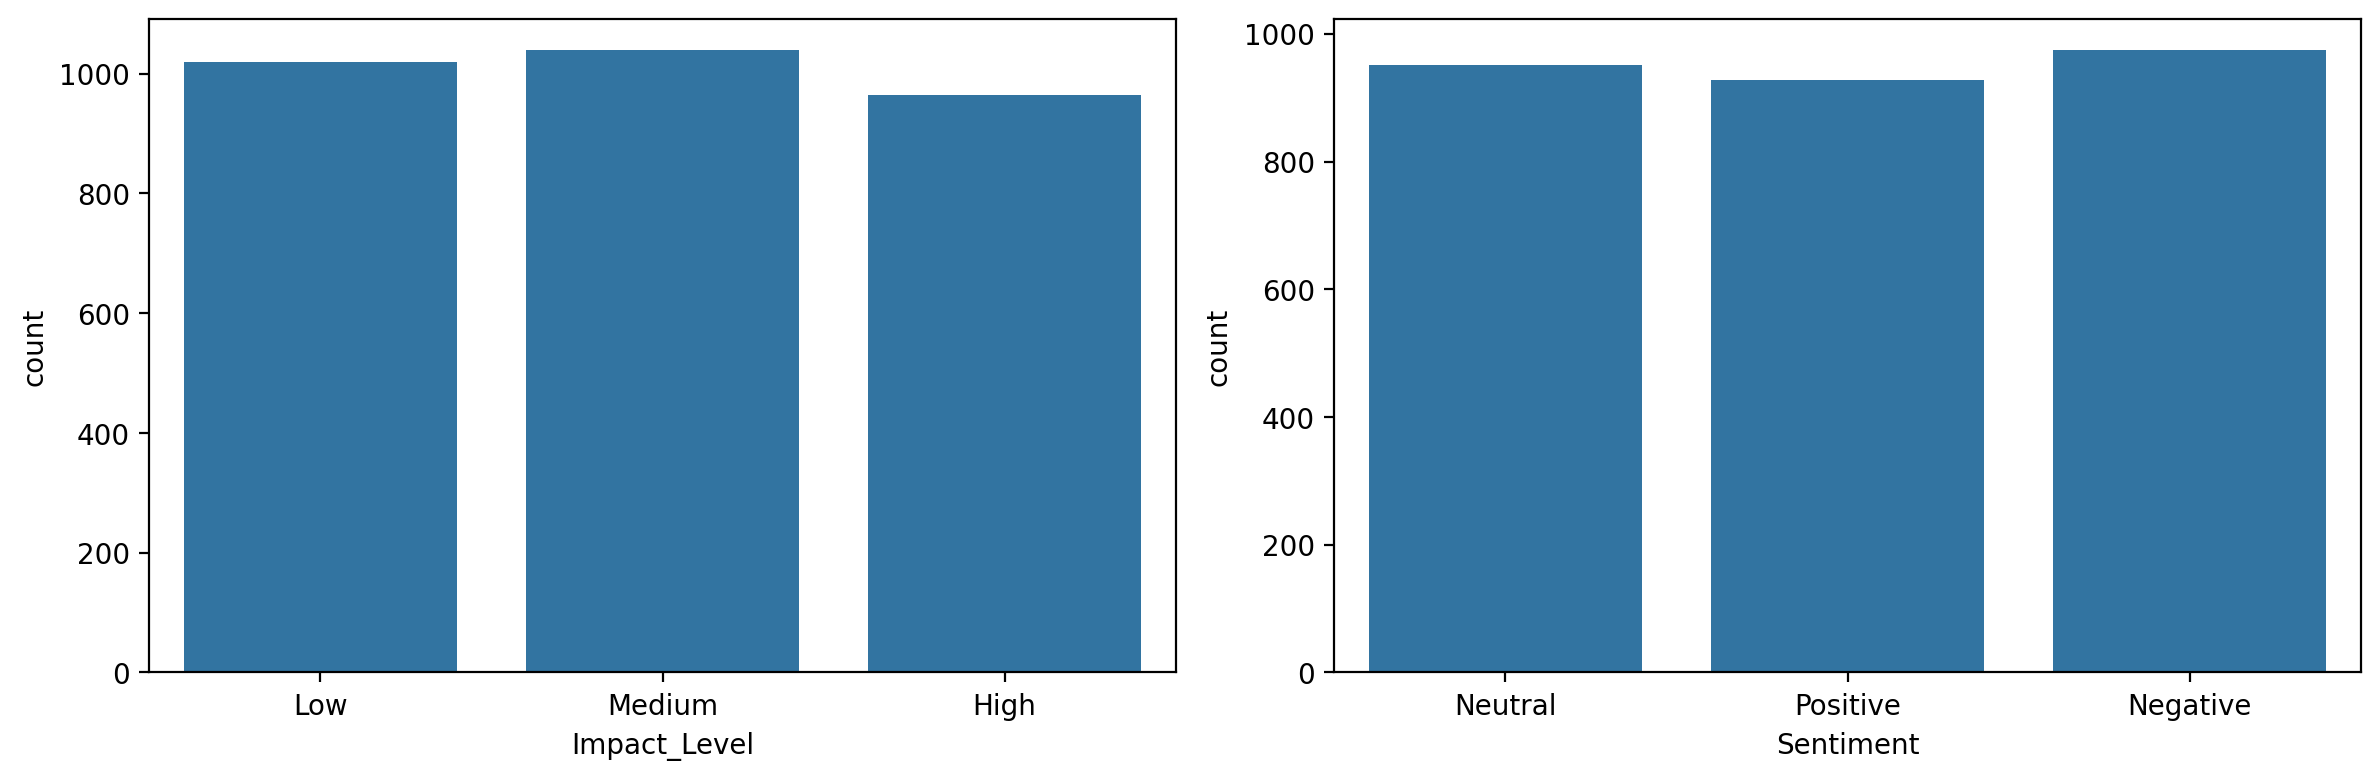
\includegraphics[width=\textwidth]{figs/eda_distribuciones.png}
\caption{Distribución de la variable objetivo (izquierda) y del sentimiento (derecha). Las tres
categorías de \texttt{Impact\_Level} y los tres valores de \texttt{Sentiment} tienen frecuencias
casi idénticas; las 171 noticias sin sentimiento registrado no aparecen en el panel derecho.}
\label{fig:distribuciones}
\end{figure}

Tras la recodificación binaria, el conjunto queda con \textbf{918 noticias de impacto alto
(31.9\,\%)} y \textbf{1{,}958 de impacto medio o bajo (68.1\,\%)}. Las clases no quedan en 50/50,
pero el desbalance es moderado y manejable. Ese 68.1\,\% es, además, el número contra el que habrá
que comparar cualquier resultado: es lo que acertaría un clasificador que respondiera siempre
``impacto medio o bajo''.

\subsection{El diagnóstico del análisis exploratorio}

La exploración del texto arroja el hallazgo que condiciona todo lo demás. En las 3{,}024 filas hay
únicamente \textbf{50 titulares distintos}, cada uno repetido en promedio 57.5 veces —entre 40 y 82
según el caso—, con una extensión media de apenas 8 palabras. El vocabulario disponible para el
clasificador es, en consecuencia, diminuto.

Más grave es lo que ocurre con las etiquetas. \textbf{Un mismo titular aparece con los tres niveles
de impacto}, y también con sentimientos y sectores distintos. Eso significa que el texto no
determina la etiqueta ni siquiera de forma aproximada, y permite calcular un techo: si a cada
titular se le asignara su nivel de impacto más frecuente —la mejor regla posible que use
únicamente el titular—, se acertaría el \textbf{41.0\,\%} de las veces, contra el 34.4\,\% de
adivinar siempre la clase mayoritaria. Siete puntos porcentuales es todo lo que el texto aporta.

El resto de las variables tampoco discrimina. La Tabla~\ref{tab:eda} muestra la proporción de cada
nivel de impacto dentro de cada sentimiento y las medias de los dos indicadores numéricos por
nivel: las distribuciones son prácticamente idénticas en los tres casos. Una noticia de sentimiento
negativo tiene la misma probabilidad de ser de impacto alto que una de sentimiento positivo, y el
cambio porcentual del índice asociado a las noticias de impacto alto no se distingue del de las de
impacto bajo.

\begin{table}[H]
\centering
\caption{Ausencia de relación entre el nivel de impacto y el resto de las variables. Arriba, la
proporción de cada nivel dentro de cada sentimiento; abajo, la media de los indicadores numéricos
por nivel.}
\label{tab:eda}
\small
\renewcommand{\arraystretch}{1.15}
\begin{tabular}{l c c c}
\toprule
\textbf{Sentimiento} & \textbf{Low} & \textbf{Medium} & \textbf{High} \\
\midrule
Negative & 0.339 & 0.337 & 0.324 \\
Neutral  & 0.331 & 0.353 & 0.315 \\
Positive & 0.345 & 0.334 & 0.321 \\
\midrule
\textbf{Nivel de impacto} & \textbf{Cambio del índice (\%)} & \textbf{Volumen (millones)} & \\
\midrule
Low    & $-0.04$ & 252.0 & \\
Medium & $+0.04$ & 253.4 & \\
High   & $-0.07$ & 241.2 & \\
\bottomrule
\end{tabular}
\end{table}

La Fig.~\ref{fig:numericas} lo muestra de forma más elocuente que la tabla: las cajas de los tres
niveles de impacto se superponen casi por completo, tanto en el cambio porcentual del índice como
en el volumen operado. Si el nivel de impacto describiera algo real del comportamiento del mercado,
la caja de las noticias de impacto alto debería estar desplazada respecto de las otras dos —más
dispersa en el cambio del índice, más alta en volumen—, y no lo está.

\begin{figure}[H]
\centering
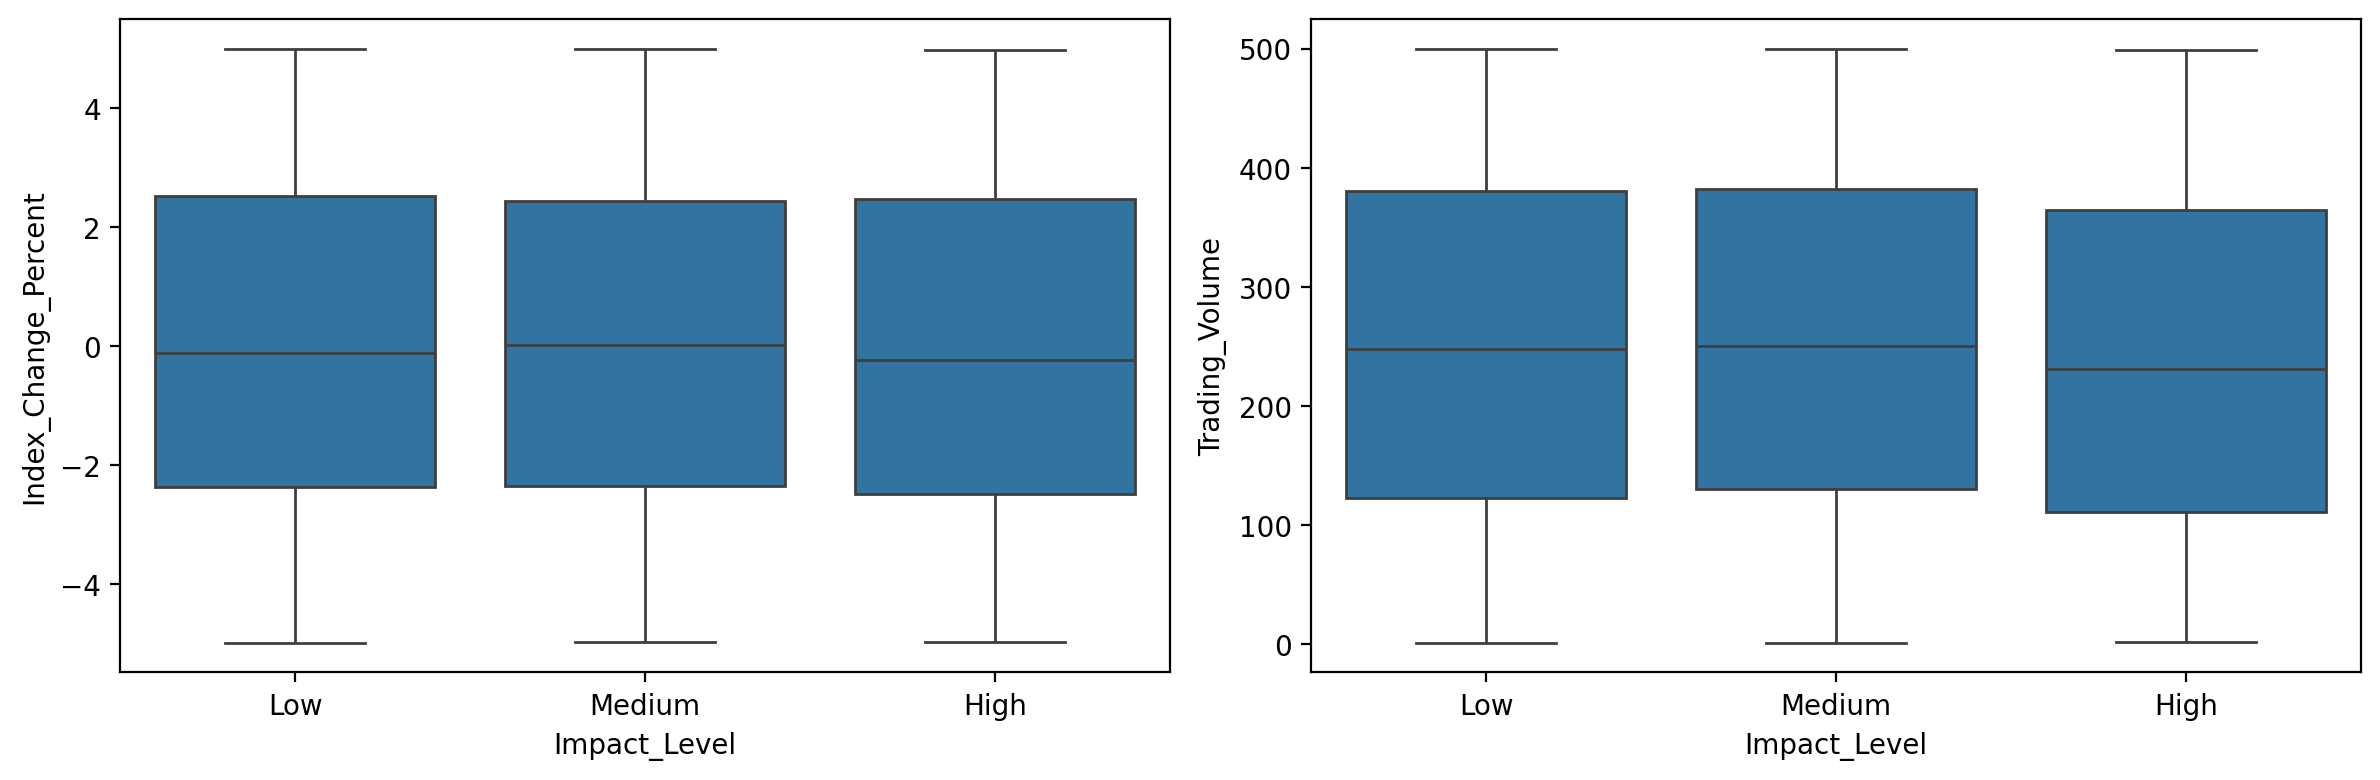
\includegraphics[width=\textwidth]{figs/eda_numericas.png}
\caption{Cambio porcentual del índice (izquierda) y volumen operado (derecha) según el nivel de
impacto declarado. Las tres distribuciones son indistinguibles entre sí, incluida la de las
noticias de impacto alto.}
\label{fig:numericas}
\end{figure}

La lectura conjunta de estos tres hechos —titulares repetidos, etiquetas contradictorias para el
mismo texto y ausencia de relación con las demás variables— apunta a que el conjunto es
\textbf{sintético y sus etiquetas fueron asignadas de forma esencialmente aleatoria}. La
consecuencia práctica es que conviene esperar un desempeño modesto del clasificador, y que un
desempeño modesto no debe interpretarse como una falla del método.

\subsection{La matriz documento--término}

Después de tokenizar y eliminar las palabras vacías, los términos más frecuentes son los que cabría
esperar de titulares financieros —\textit{market}, \textit{sector}, \textit{stocks},
\textit{trade}, \textit{investors}—, lo que confirma que la limpieza conservó vocabulario con
contenido y no residuos gramaticales.

La matriz resultante tiene \textbf{2{,}876 renglones y 238 columnas}, con \textbf{18{,}248 entradas
distintas de cero}, es decir una densidad de \textbf{2.67\,\%}. Un vocabulario de 238 términos es
muy pequeño para clasificación de texto, y es la traducción directa de tener solo 50 titulares
distintos de ocho palabras cada uno. El vector de etiquetas tiene la misma longitud que el número
de renglones y está ordenado por el mismo identificador, de modo que cada fila conserva su
etiqueta.

\subsection{Entrenamiento y resultados}

La partición deja \textbf{2{,}301 registros de entrenamiento y 575 de prueba}, con proporciones de
clase similares entre ambos, de modo que el muestreo aleatorio no introdujo un desbalance
adicional. La Tabla~\ref{tab:confusion} presenta la matriz de confusión sobre el conjunto de prueba
y la Tabla~\ref{tab:metricas} las métricas que se derivan de ella.

\begin{table}[H]
\centering
\caption{Matriz de confusión sobre el conjunto de prueba ($n = 575$).}
\label{tab:confusion}
\small
\renewcommand{\arraystretch}{1.2}
\begin{tabular}{l c c c}
\toprule
& \multicolumn{2}{c}{\textbf{Predicho}} & \\
\cmidrule(lr){2-3}
\textbf{Real} & \textbf{Impacto Alto} & \textbf{Impacto Otro/Bajo} & \textbf{Total} \\
\midrule
Impacto Alto      & 86  & 95  & 181 \\
Impacto Otro/Bajo & 172 & 222 & 394 \\
\midrule
\textbf{Total}    & 258 & 317 & 575 \\
\bottomrule
\end{tabular}
\end{table}

\begin{table}[H]
\centering
\caption{Métricas de desempeño, tomando \texttt{Impacto Alto} como clase positiva.}
\label{tab:metricas}
\small
\renewcommand{\arraystretch}{1.15}
\begin{tabular}{l c l}
\toprule
\textbf{Métrica} & \textbf{Valor} & \textbf{Referencia} \\
\midrule
Exactitud     & 0.536 & Línea base (clase mayoritaria): \textbf{0.685} \\
Precisión     & 0.333 & Azar bajo la proporción de la clase: 0.315 \\
Sensibilidad  & 0.475 & --- \\
$F_1$         & 0.392 & --- \\
\bottomrule
\end{tabular}
\end{table}

El modelo alcanza una exactitud de \textbf{53.6\,\%}, \textbf{por debajo del 68.5\,\%} que se
obtendría prediciendo siempre la clase mayoritaria. No es solo que aprenda poco: en términos de
exactitud, aplicarlo es peor que no tener modelo. La precisión de 33.3\,\% apenas se distingue de
la proporción de noticias de impacto alto en el conjunto de prueba, que es lo que obtendría un
clasificador que lanzara alertas al azar. La sensibilidad de 47.5\,\% completa el cuadro: el
modelo se comporta, en la práctica, como si estuviera decidiendo por sorteo.

\subsection{Interpretación en el contexto financiero}

Las dos formas de equivocarse tienen costos distintos para quien invierte, y conviene traducirlas.

\textbf{Falsas alarmas.} El modelo emite 258 alertas de impacto alto y solo 86 son correctas: de
cada tres alertas, dos son falsas. Un inversionista que actuara sobre cada una estaría
cubriéndose, vendiendo o reposicionándose ante noticias que no iban a mover el mercado, y pagaría
comisiones y fricción casi el doble de veces de las que acertaría. Más allá del costo directo, una
señal que se equivoca dos de cada tres veces pierde credibilidad y deja de usarse.

\textbf{Oportunidades perdidas.} De las 181 noticias de impacto alto que realmente ocurrieron en el
conjunto de prueba, 95 —el 52.5\,\%— quedaron clasificadas como impacto medio o bajo. Más de la
mitad de las noticias relevantes pasan desapercibidas, lo que deja al inversionista sin cobertura
frente a movimientos reales del mercado justamente cuando la necesitaría.

Con este desempeño el modelo no es utilizable en ninguno de los dos extremos: no sirve como
sistema de alerta, porque satura de falsos positivos, ni como filtro de tranquilidad, porque deja
pasar la mitad de lo importante. Y conviene subrayar de dónde viene el problema. Un clasificador
cuyo techo, usando el texto disponible, es del 41\,\% en la tarea de tres clases no puede rendir
mucho más; el ruido en las etiquetas acota el desempeño alcanzable con independencia del algoritmo
\cite{frenay2014}, y ninguna elección de modelo recupera información que los datos no contienen.
Cambiar naïve Bayes por un método más sofisticado no cambiaría el diagnóstico: el error
irreducible del problema, tal como está planteado, es demasiado alto \cite{hastie2009}.

\subsection{Limitaciones}

\textbf{El conjunto no permite aprender.} Es la limitación dominante y no es del método: 50
titulares distintos, cada uno repetido decenas de veces y etiquetado de forma inconsistente, dejan
al clasificador sin señal que extraer. Los resultados de este trabajo describen ese conjunto, no la
capacidad de naïve Bayes para clasificar noticias financieras en general.

\textbf{Falta de documentación del origen de los datos.} No se dispone de información sobre cómo se
generaron las noticias ni sobre cómo se asignaron las etiquetas de impacto, que es justamente lo
que permitiría confirmar la sospecha de que el conjunto es sintético. La práctica de acompañar cada
conjunto con una ficha que documente su procedencia y su proceso de etiquetado existe precisamente
para evitar este tipo de ambigüedad \cite{gebru2021}.

\textbf{Supuesto de independencia sobre titulares muy cortos.} Con una media de ocho palabras por
titular, y tras eliminar las vacías, quedan pocos términos por documento; el supuesto de
independencia condicional se vuelve más frágil cuando cada palabra pesa mucho en el producto de
\eqref{eq:nb}.

\textbf{Una sola partición.} Las métricas provienen de una única división en entrenamiento y
prueba. Un esquema de validación cruzada daría una estimación más estable, aunque con este nivel de
desempeño la conclusión difícilmente cambiaría.

\textbf{Solo se usó el texto.} El modelo se entrena únicamente con la matriz de titulares; el
sentimiento, el sector, el evento de mercado y los indicadores numéricos se conservaron en el
conjunto analítico pero no entraron al clasificador. El análisis exploratorio sugiere que
incorporarlos no habría ayudado, ya que ninguno discrimina entre niveles de impacto, pero eso no se
verificó ajustando un modelo con ellos.

% ─── 4. CONCLUSIONES ──────────────────────────────────────────────────────────
\section{Conclusiones}

El trabajo se planteó una pregunta directa: si un clasificador naïve Bayes multinomial puede
decidir, a partir del titular, si una noticia financiera va a mover el mercado de forma apreciable.
La respuesta, para el conjunto analizado, es que no. El modelo se comporta peor que la regla
trivial de responder siempre la categoría más común, emite bastantes más alertas falsas que
correctas y deja pasar más de la mitad de las noticias que sí eran relevantes, de modo que no
sirve ni como sistema de aviso ni como filtro de tranquilidad. Un inversionista que actuara sobre
sus señales pagaría fricción por operaciones innecesarias y, al mismo tiempo, quedaría sin
cobertura frente a buena parte de los movimientos reales.

Lo interesante es que ese resultado estaba anunciado antes de entrenar nada. La exploración de los
datos mostró que el conjunto contiene muy pocos titulares distintos, repetidos muchas veces, y que
un mismo titular aparece etiquetado con todos los niveles de impacto; que el sentimiento no
distingue unas noticias de otras; y que los indicadores del índice y del volumen se distribuyen
igual sin importar el impacto declarado. Con esas tres observaciones sobre la mesa, la mejor regla
concebible que use solamente el texto apenas mejora al azar, y ningún clasificador puede superar un
techo que fijan los datos y no el algoritmo. La conclusión metodológica es más valiosa que la
métrica: cuando el desempeño es bajo conviene averiguar si el problema está en el modelo o en el
conjunto antes de cambiar de método, porque en el segundo caso ningún cambio de método ayuda.

Al mismo tiempo, el flujo construido sí cumplió su función. Las decisiones de limpieza se tomaron
variable por variable y quedaron escritas, la recodificación de la variable objetivo respondió a
una lógica operativa —lo que le importa a quien invierte es separar lo que mueve el mercado de lo
que no—, la representación del texto siguió el camino habitual de tokenizar, descartar palabras
vacías y construir una matriz dispersa de conteos, y el suavizado evitó que una palabra
desconocida anulara una clase entera. Ese andamiaje es reutilizable tal cual, y esa es la parte del
trabajo que sobrevive al conjunto de datos con el que se probó.

De cara a lo que sigue, el camino evidente es sustituir la fuente por titulares reales y variados,
con etiquetas de impacto derivadas del comportamiento observado del índice en lugar de asignadas de
antemano; con eso el mismo flujo produciría una evaluación informativa, favorable o no. Sobre esa
base tendría sentido incorporar al clasificador las variables que aquí se conservaron pero no se
usaron, comparar la representación de conteos contra alternativas que ponderen los términos por su
capacidad de discriminar, y sustituir la partición única por validación cruzada para que las
métricas vengan con una medida de su variabilidad. Ninguna de esas mejoras tiene sentido, sin
embargo, mientras las etiquetas no guarden relación con el texto: la primera tarea de cualquier
continuación es conseguir datos que sí contengan la señal que se pretende aprender.

% ─── REFERENCIAS ──────────────────────────────────────────────────────────────
\begin{thebibliography}{99}
\small

\bibitem{tetlock2007} Tetlock, P. C. (2007). Giving content to investor sentiment: The role of
media in the stock market. \textit{The Journal of Finance}, 62(3), 1139--1168.

\bibitem{loughran2011} Loughran, T., \& McDonald, B. (2011). When is a liability not a liability?
Textual analysis, dictionaries, and 10-Ks. \textit{The Journal of Finance}, 66(1), 35--65.

\bibitem{antweiler2004} Antweiler, W., \& Frank, M. Z. (2004). Is all that talk just noise? The
information content of internet stock message boards. \textit{The Journal of Finance}, 59(3),
1259--1294.

\bibitem{manning2008} Manning, C. D., Raghavan, P., \& Schütze, H. (2008). \textit{Introduction to
Information Retrieval}. Cambridge: Cambridge University Press.

\bibitem{mccallum1998} McCallum, A., \& Nigam, K. (1998). A comparison of event models for naive
Bayes text classification. En \textit{AAAI-98 Workshop on Learning for Text Categorization},
41--48.

\bibitem{domingos1997} Domingos, P., \& Pazzani, M. (1997). On the optimality of the simple
Bayesian classifier under zero-one loss. \textit{Machine Learning}, 29(2--3), 103--130.

\bibitem{frenay2014} Frénay, B., \& Verleysen, M. (2014). Classification in the presence of label
noise: A survey. \textit{IEEE Transactions on Neural Networks and Learning Systems}, 25(5),
845--869.

\bibitem{mckinney2010} McKinney, W. (2010). Data structures for statistical computing in Python.
En \textit{Proceedings of the 9th Python in Science Conference}, 56--61.

\bibitem{rcore2024} R Core Team (2024). \textit{R: A Language and Environment for Statistical
Computing}. Viena: R Foundation for Statistical Computing.

\bibitem{wickham2019} Wickham, H., et al.\ (2019). Welcome to the tidyverse. \textit{Journal of
Open Source Software}, 4(43), 1686.

\bibitem{silge2016} Silge, J., \& Robinson, D. (2016). tidytext: Text mining and analysis using
tidy data principles in R. \textit{Journal of Open Source Software}, 1(3), 37.

\bibitem{majka2019} Majka, M. (2019). \textit{naivebayes: High Performance Implementation of the
Naive Bayes Algorithm in R}. Paquete de R.

\bibitem{rubin1976} Rubin, D. B. (1976). Inference and missing data. \textit{Biometrika}, 63(3),
581--592.

\bibitem{hastie2009} Hastie, T., Tibshirani, R., \& Friedman, J. (2009). \textit{The Elements of
Statistical Learning} (2a ed.). Nueva York: Springer.

\bibitem{gebru2021} Gebru, T., Morgenstern, J., Vecchione, B., Vaughan, J. W., Wallach, H.,
Daumé III, H., \& Crawford, K. (2021). Datasheets for datasets. \textit{Communications of the ACM},
64(12), 86--92.

\end{thebibliography}

\end{document}
